\ifx\PREAMBLE\UnDef
\documentclass{beamer}
\usepackage{tikz}
\usetikzlibrary{shapes,arrows,snakes}

\usepackage[english]{babel}
% or whatever

\usepackage[latin1]{inputenc}
% or whatever

\usepackage[T1]{fontenc}
\usepackage{amssymb}
\usepackage{amsmath}
\usepackage{eventB}
\newBvrb[trains]{trns}
\newBevt{arrives}
\newBevt{departs}

\begin{document}
\else
\fi


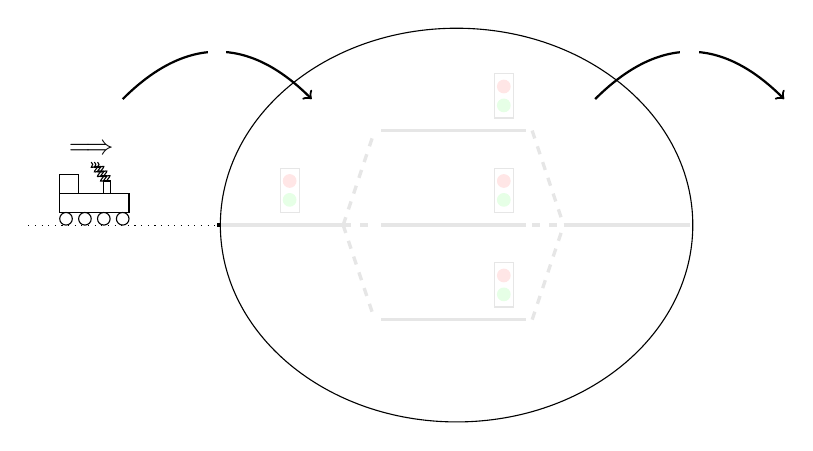
\begin{tikzpicture}[scale=0.8]
  \uncover<1,2>{
    % approaching block.
    \draw[very thick] (0,0) -- (1.5,0);
%    \draw (0.7, -1) node{entry block};
    
    % in-switch
    \draw[very thick] (1.5,0) -- (2,0);
    \draw[very thick, dashed] (2,0) -- (2.5,1.5);
    \draw[very thick, dashed] (2,0) -- (2.5,-1.5);
    \draw[very thick, dashed] (2,0) -- (2.5,0);
    % \draw[red] (2, -1.5) node{in-switch};
    
    % platform blocks
    \draw[very thick] (2.6,0) -- (4.9,0);
    % \draw[very thick, dotted] (2.6,0.5) -- (4.9,0.5);
    % \draw[very thick, dotted] (2.6,-0.5) -- (4.9,-0.5);
    \draw[very thick] (2.6,1.5) -- (4.9,1.5);
    \draw[very thick] (2.6,-1.5) -- (4.9,-1.5);
%    \draw (3.75, -2.5) node{platform blocks};
    
    % out-switch
    \draw[very thick] (5.5,0) -- (6,0);
    \draw[very thick, dashed] (5,1.5) -- (5.5,0);
    \draw[very thick, dashed] (5,0) -- (5.5,0);
    \draw[ very thick, dashed] (5,-1.5) -- (5.5,0);
    % \draw[red] (5.5, -1.5) node{out-switch};
    
    % exiting block.
    \draw[very thick] (6.0,0) -- (7.5,0);
%    \draw (6.8, -1) node{exit block};
    
    % entry signal
    % \draw[very thick] (1.45,0) -- (1.45, 1);
    \draw (1, 0.2) rectangle +(0.3,0.7);
    \filldraw[red] (1.15, 0.7) circle (0.1);
    \filldraw[green] (1.15, 0.4) circle (0.1);
%    \draw (1.15, 1.2) node{entry signal};
    
    % platform signals
    % \draw[very thick] (6.05,0) -- (6.05, 1);
    \draw (4.4, 0.2) rectangle +(0.3,0.7);
    \filldraw[red] (4.55, 0.7) circle (0.1);
    \filldraw[green] (4.55, 0.4) circle (0.1);
%    \draw (4.55, 2.9) node{platform signals};
    
    \draw (4.4, 1.7) rectangle +(0.3,0.7);
    \filldraw[red] (4.55, 2.2) circle (0.1);
    \filldraw[green] (4.55, 1.9) circle (0.1);
    
    \draw (4.4, -1.3) rectangle +(0.3,0.7);
    \filldraw[red] (4.55, -0.8) circle (0.1);
    \filldraw[green] (4.55, -1.1) circle (0.1);
  }

  % The train
  \draw[dotted] (-3,0) -- (0, 0);
  \draw(-2.5,0.2) rectangle +(1.1, 0.3);
  \draw(-2.5,0.5) rectangle +(0.3, 0.3);
  \draw(-1.8,0.5) rectangle +(0.1, 0.2);
  \draw[decorate, decoration={snake, amplitude = 1pt, segment length = 2pt}] (-1.8,0.7) --  (-2,1);
  \draw[decorate, decoration={snake, amplitude = 1pt, segment length = 2pt}] (-1.75,0.7) --  (-1.95,1);
  \draw[decorate, decoration={snake, amplitude = 1pt, segment length = 2pt}] (-1.7,0.7) --  (-1.9,1);
  \draw (-2.4, 0.1) circle (0.1);
  \draw (-2.1, 0.1) circle (0.1);
  \draw (-1.8, 0.1) circle (0.1);
  \draw (-1.5, 0.1) circle (0.1);
  \draw (-2, 1.2) node{$\Longrightarrow$};
  
  \uncover<2->{
    \draw (3.8,0) node[fill opacity=.9, fill=white, ellipse, draw, minimum width = 6cm, minimum height = 5cm]{};
    
    \draw[thick,->] (-1.5,2) .. controls (-0.5,3) and (0.5,3)  ..node[fill=white]{\arrives} (1.5,2);

    \draw (3.8,2.5) node{\trains};
  
    \draw[thick,->] (6,2) .. controls (7,3) and (8,3)  ..node[fill=white]{\departs} (9,2);
  }
\end{tikzpicture}

\ifx\PREAMBLE\UnDef
\end{document}
\else
\fi
